\chapter{LITERATURE SURVEY}
\patchcmd{\chapter}{\thispagestyle{fancy}}{}{}
  \hrulefill\\
  \thispagestyle{empty}
\renewcommand{\thesection}{\thechapter.\arabic{section}}
  \doublespacing
  \section{Introduction}
 {%\noindent
  In today’s competitive job market, organizations receive a large number of resumes for every job opening, making manual screening a time-consuming and inefficient process. Traditional recruitment methods often rely on keyword matching and human judgment, which can lead to inconsistencies, bias, and missed opportunities to identify suitable candidates. With the rapid growth of Natural Language Processing (NLP), automated resume analysis systems have emerged as an effective solution to streamline recruitment. These systems are capable of extracting relevant information such as skills, education, and experience, and matching it with job descriptions to identify the most suitable candidates. By leveraging advanced NLP techniques and machine learning models, resume analysis systems not only improve efficiency but also enhance accuracy and fairness in the hiring process.}

\section{Literature Survey}
{%\noindent
Several research studies have explored the use of NLP and machine learning techniques for automated resume analysis. Early systems relied on rule-based and keyword-matching approaches, which lacked the ability to understand context and semantics. To overcome these limitations, machine learning models such as Support Vector Machines and Decision Trees were introduced, improving classification accuracy but still requiring manual feature extraction. With the advancement of deep learning, techniques like Named Entity Recognition (NER) have been widely used to extract structured data such as names, skills, and qualifications from resumes using tools like spaCy and NLTK. Furthermore, transformer-based models such as BERT have significantly improved semantic understanding, enabling systems to analyze the meaning of text rather than relying solely on keywords. Recent research also incorporates Retrieval-Augmented Generation (RAG) models to provide explanations, feedback, and better matching between resumes and job descriptions. Despite these advancements, existing systems still face challenges such as bias, lack of explainability, and difficulty handling diverse resume formats.}

Several research studies have explored the use of Natural Language Processing (NLP) and machine learning techniques for automated resume analysis. Early systems primarily relied on rule-based methods and keyword matching, which were simple to implement but lacked the ability to understand contextual meaning, resulting in poor generalization and inaccurate candidate screening. These systems often failed when synonyms or varied phrasing were used, limiting their effectiveness in real-world scenarios.

To address these limitations, traditional machine learning models such as Support Vector Machines (SVM), Naïve Bayes, and Decision Trees were introduced. These approaches improved classification performance by learning patterns from data; however, they still depended heavily on manual feature engineering, such as extracting keywords, term frequency–inverse document frequency (TF-IDF), and syntactic features. This process was time-consuming and required domain expertise, making the systems less scalable and adaptable.
\newpage
\begin{figure}[h]
\centering
 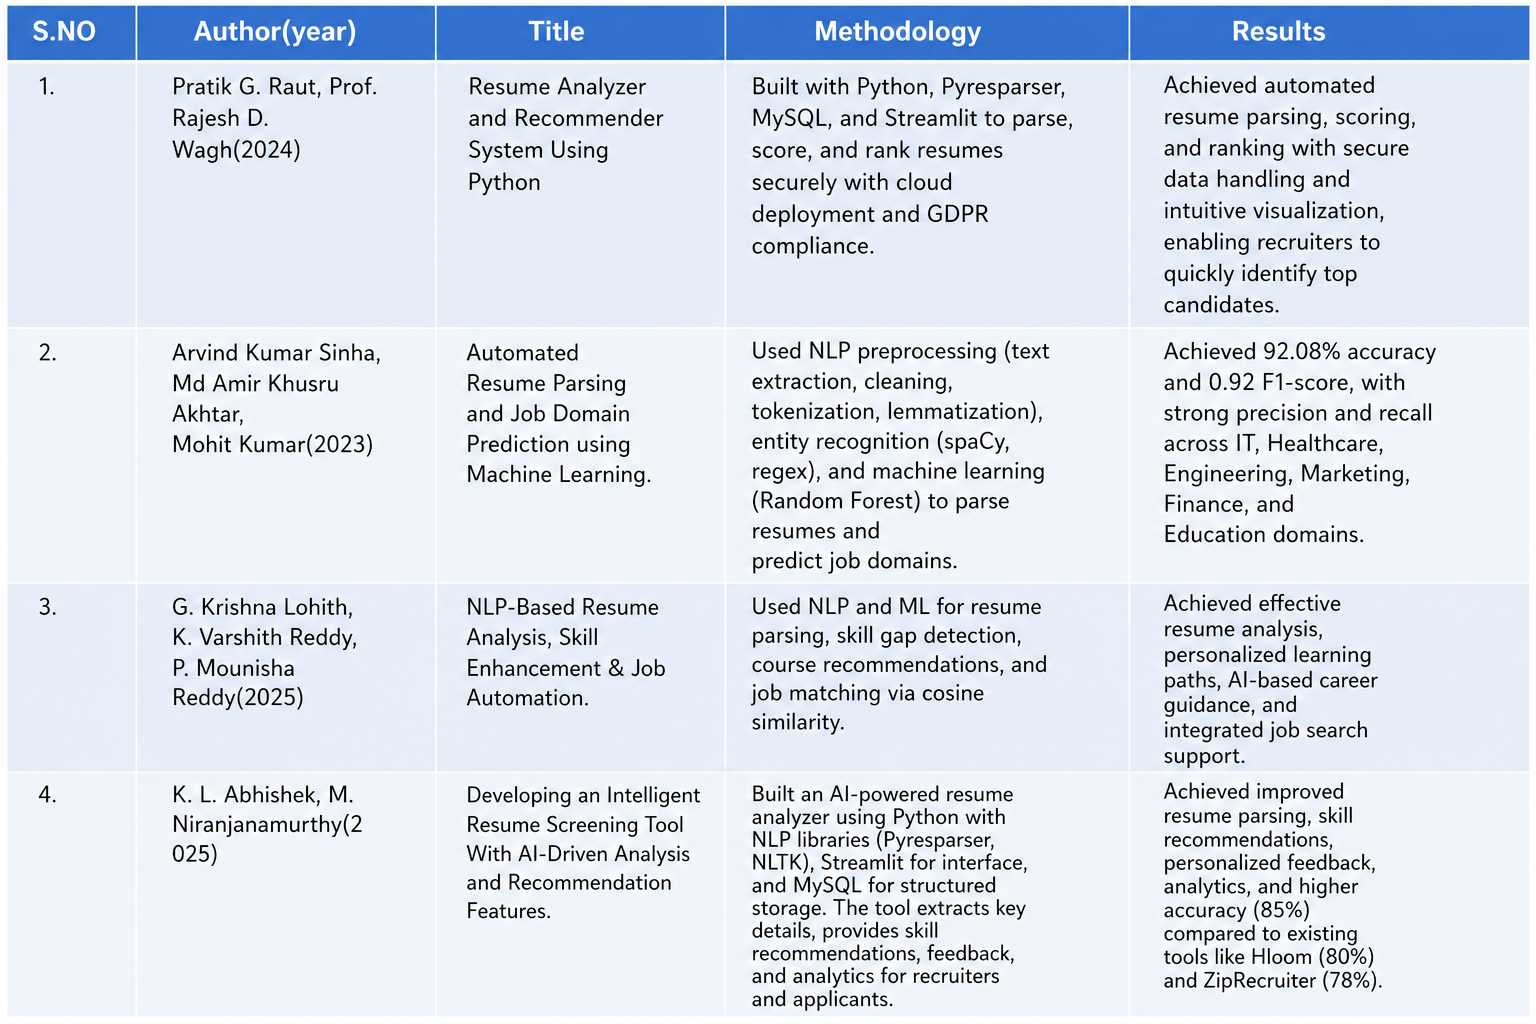
\includegraphics[width=1.1\textwidth]{images/Literature Survey.png}
 \captionof{figure}{Literature survey} 
\end{figure}

\newpage
\section{Summary}
{%\noindent}
In summary, the evolution of resume analysis systems has progressed from simple keyword-based methods to advanced NLP and deep learning models capable of understanding context and semantics. While modern approaches using techniques like NER, transformer models, and RAG have significantly improved accuracy and efficiency, there remain gaps in terms of transparency, fairness, and adaptability. The proposed system aims to address these limitations by integrating multiple techniques, including resume parsing, semantic matching, and feedback generation, to create a more robust and intelligent recruitment solution. This approach not only enhances candidate-job matching but also provides meaningful insights and guidance to applicants, ultimately improving the overall recruitment process, while also ensuring scalability for handling large volumes of resumes and enabling continuous learning to adapt to evolving job market trends.}



\begin{figure}[h]
\centering
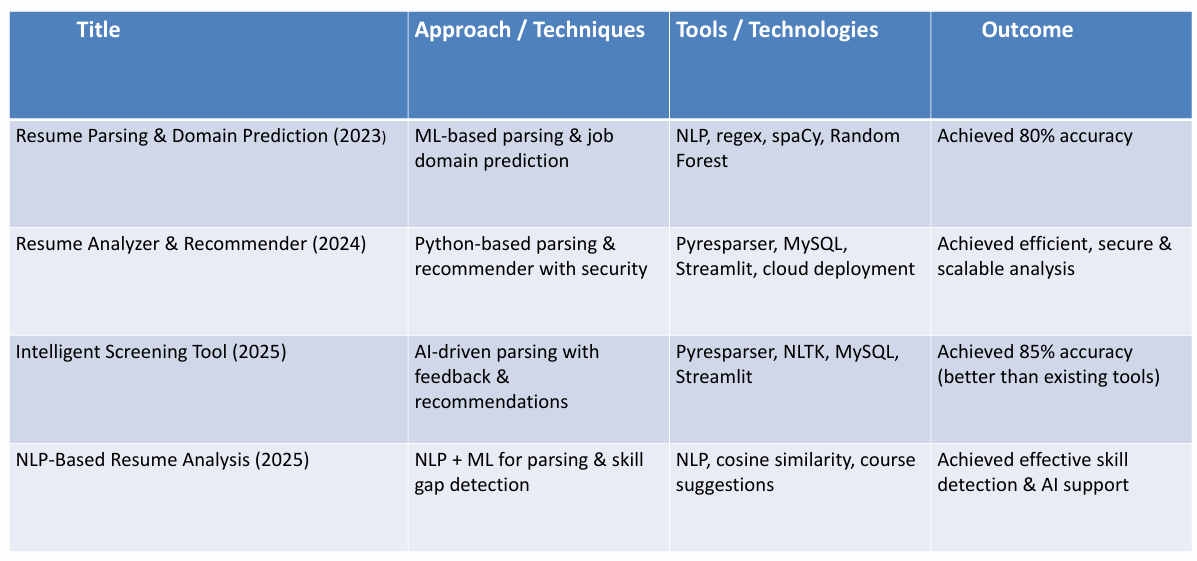
\includegraphics[width=1.1\textwidth]{chapters/Screenshot 2026-04-29 090934.png}
 \captionof{figure}{Comparsion Table} 
\end{figure}
{%\noindent
The three papers illustrate the evolution of resume analysis systems from basic parsing and ranking (2024), to more accurate prediction using NLP and ML techniques like Random Forest (2023), and finally to advanced AI-driven systems (2025) that include skill gap detection, course recommendations, and job matching. The later approaches improve accuracy, automation, and user experience. Overall, this progression highlights a shift toward intelligent, efficient, and personalized recruitment solutions that benefit both recruiters and job seekers.}
